% Loss Function
\subsection{Loss Function}

One key aspect of NNs is to \textit{learn} by training with multiple examples. This process of learning is done by making a prediction $\hat{y}$ and then comparing it to the \textbf{ground truth} $y$. The error is then the difference between these two values, figure \ref{fig:errors} depicts these differences. 

The \textbf{loss function} $L(Y, f(X))$ is "a function for penalizing the errors in prediction" \cite{Hastie2009ElementsLearning}. This function is also called the \textbf{cost function}, \textbf{objective function}, or \textbf{error function}. The objective is to minimize or maximize such function, it is usually denoted by a superscript $\ast$. For example, $x^{\ast}= arg min f(x)$ \cite{Goodfellow.Ian2016DeepLearning}. The robustness of the model increases when the value of the loss function decreases. \cite{LossChanghau}

% FIGURE: ANN Architecture
\begin{figure}[!htb]	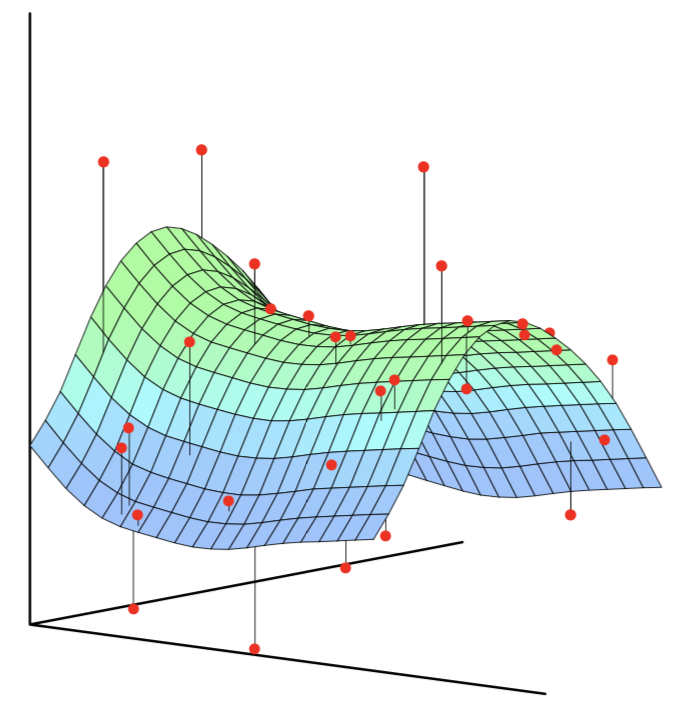
\includegraphics[width=0.5\textwidth]{images/errors.png} 
    \centering

\caption{
The error is the difference between the real value $y$ (red dots) and the predicted values $\hat{y}$ (values in the function). \cite{HastieSpringerLearning}
} 

\label{fig:errors}
\end{figure}
Loss function is one of the most important aspects of NNs. There exists many loss functions and many more are being developed. The following list is not an extensive or exhaustive list but rather an introduction of the most common loss functions.

% MSE
\subsubsection{Mean Squared Error}
The \textbf{Mean Squared Error (MSE)} is a loss function whose objective is to minimize the residual sum of squares. This loss function is very popular because it is the easiest measure to manipulate mathematically \cite{Witten2011DataTechniques}. The objective is to fit a line such that this optimized line minimizes the sum of distance of each point to the regression line.

\begin{equation} \label{eq:loss-mse}
	\boldsymbol{\mathcal{L}}=\frac{1}{n}\sum_{i=1}^{n}(y^{(i)}-\hat{y}^{(i)})^{2}
\end{equation}

% MAE
\subsubsection{Mean Absolute Error}
\textbf{Mean Absolute Error (MAE)} outputs the relative errors. The key difference between MSE and MAE is that MSE exaggerates the effect of outliers but MAE does not have this effect. In MAE, errors are treated evenly in accordance to their value. \cite{Witten2011DataTechniques}

\begin{equation} \label{eq:loss-mae}
	\boldsymbol{\mathcal{L}}=\frac{1}{n}\sum_{i=1}^{n}\big\lvert y^{(i)}-\hat{y}^{(i)}\big\rvert
\end{equation}


% L2
\subsubsection{L2}
\textbf{L2} loss function is the square of the L2 norm of the difference between ground truth and prediction. It is quite similar to MSE, except it does not have a division by $n$.

\begin{equation} \label{eq:loss-l2}
	\boldsymbol{\mathcal{L}}=\sum_{i=1}^{n}(y^{(i)}-\hat{y}^{(i)})^{2}
\end{equation}

% Cross Entropy
\subsubsection{Cross Entropy}
\textbf{Cross Entropy} is commonly-used in binary classification (labels are assumed to take values 0 or 1) as a loss function (For multi-classification, use Multi-class Cross Entropy. Cross entropy measures the divergence between two probability distribution.

\begin{equation} \label{eq:loss-crossentropy}
	\boldsymbol{\mathcal{L}}=-\frac{1}{n}\sum_{i=1}^{n}\big[y^{(i)}\log(\hat{y}^{(i)})+(1-y^{(i)})\log(1-\hat{y}^{(i)})\big]
\end{equation}

% Hinge Loss
\subsubsection{Hinge Loss}
\textbf{Hinge Loss}, also known as max-margin objective, is a loss function used for training classifiers. The hinge loss is used for “maximum-margin” classification.

\begin{equation} \label{eq:loss-hinge}
	\boldsymbol{\mathcal{L}}=\frac{1}{n}\sum_{i=1}^{n}\max(0,1-y^{(i)}\cdot\hat{y}^{(i)})
\end{equation}
